\documentclass[11pt,a4paper]{article}
\usepackage[spanish,es-nodecimaldot]{babel}	% Utilizar español
\usepackage[utf8]{inputenc}					% Caracteres UTF-8
\usepackage{graphicx}						% Imagenes
\usepackage[hidelinks]{hyperref}			% Poner enlaces sin marcarlos en rojo
\usepackage{fancyhdr}						% Modificar encabezados y pies de pagina
\usepackage{float}							% Insertar figuras
\usepackage[textwidth=390pt]{geometry}		% Anchura de la pagina
\usepackage[nottoc]{tocbibind}				% Referencias (no incluir num pagina indice en Indice)
\usepackage{enumitem}						% Permitir enumerate con distintos simbolos
\usepackage[T1]{fontenc}					% Usar textsc en sections
\usepackage{amsmath}						% Símbolos matemáticos
\usepackage{natbib}
\usepackage{subcaption}

% Comando para poner el nombre de la asignatura
\newcommand{\asignatura}{Visión por Computador}
\newcommand{\autor}{Vladislav Nikolov Vasilev}
\newcommand{\titulo}{Práctica 3}
\newcommand{\subtitulo}{Detección de puntos relevantes y Construcción de panoramas}

\usepackage{listings}
\usepackage{xcolor}
 
\definecolor{codegreen}{rgb}{0,0.6,0}
\definecolor{codegray}{rgb}{0.5,0.5,0.5}
\definecolor{codepurple}{rgb}{0.58,0,0.82}
\definecolor{backcolour}{rgb}{0.95,0.95,0.92}
 
\lstdefinestyle{mystyle}{
    backgroundcolor=\color{backcolour},   
    commentstyle=\color{codegreen},
    keywordstyle=\color{magenta},
    numberstyle=\tiny\color{codegray},
    stringstyle=\color{codepurple},
    basicstyle=\ttfamily\footnotesize,
    breakatwhitespace=false,         
    breaklines=true,                 
    captionpos=b,                    
    keepspaces=true,                 
    numbers=left,                    
    numbersep=5pt,                  
    showspaces=false,                
    showstringspaces=false,
    showtabs=false,                  
    tabsize=4,
    language=Python,
    literate={ñ}{{\~n}}1
}

\lstset{style=mystyle}


% Configuracion de encabezados y pies de pagina
\pagestyle{fancy}
\lhead{\autor{}}
\rhead{\asignatura{}}
\lfoot{Grado en Ingeniería Informática}
\cfoot{}
\rfoot{\thepage}
\renewcommand{\headrulewidth}{0.4pt}		% Linea cabeza de pagina
\renewcommand{\footrulewidth}{0.4pt}		% Linea pie de pagina

\begin{document}
\pagenumbering{gobble}

% Pagina de titulo
\begin{titlepage}

\begin{minipage}{\textwidth}

\centering

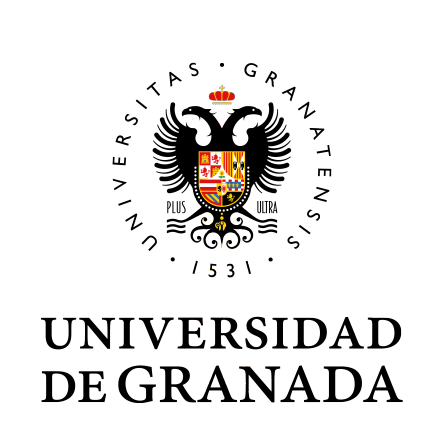
\includegraphics[scale=0.5]{img/ugr.png}\\

\textsc{\Large \asignatura{}\\[0.2cm]}
\textsc{GRADO EN INGENIERÍA INFORMÁTICA}\\[1cm]

\noindent\rule[-1ex]{\textwidth}{1pt}\\[1.5ex]
\textsc{{\Huge \titulo\\[0.5ex]}}
\textsc{{\large \subtitulo\\}}
\noindent\rule[-1ex]{\textwidth}{2pt}\\[3.5ex]

\end{minipage}

\vspace{0.5cm}

\begin{minipage}{\textwidth}

\centering

\textbf{Autor}\\ {\autor{}}\\[2.5ex]
\textbf{Rama}\\ {Computación y Sistemas Inteligentes}\\[2.5ex]
\vspace{0.3cm}


\includegraphics[scale=0.3]{img/etsiit.jpeg}

\vspace{0.7cm}
\textsc{Escuela Técnica Superior de Ingenierías Informática y de Telecomunicación}\\
\vspace{1cm}
\textsc{Curso 2019-2020}
\end{minipage}
\end{titlepage}

\pagenumbering{arabic}
\tableofcontents
\thispagestyle{empty}				% No usar estilo en la pagina de indice

\newpage

\setlength{\parskip}{1em}

\section{\textsc{Detección de puntos Harris}}

En esta primera sección vamos a estudiar el comportamiento del detector de
puntos Harris, y cómo podemos utilizarlo para extraer \textit{keypoints} de la
imagen. Para ello, vamos a implementar algunas funciones que simulen
el comportamiento de las de \texttt{OpenCV}. Además, vamos a experimentar
con los parámetros que reciben dichas funciones para ver cómo se ve afectada
la salida. Finalmente, vamos a refinar un poco los puntos que hemos obtenido,
para ver cómo de buenas son las estimaciones que hemos hecho.

\subsection{Estimación de los \textit{keypoints} utilizando Harris}

Nuestro principal objetivo es, dada una imagen en escala de grises,
obtener los \textit{keypoints}, los cuáles pueden ser utilizados para
otras muchas cosas, como por ejemplo para el \textit{matching} entre
imágenes. Existen muchos operadores que podemos utilizar para extraer
los \textit{keypoints}, pero nosotros aquí vamos a utilizar el operador
de Harris, y lo combinaremos con algunas técnicas más. Es importante
recalcar la parte de \textbf{imagen en escala de grises}, ya que Harris
solo funciona con imágenes de este tipo.

Harris se utiliza principalmente para extraer las esquinas de una
imagen. Aprovechando dicha información, podemos sacar información
relevante que sea representativa de la imagen que tenemos a diversas escalas,
de forma que en un principio nos fijamos en qué se encuentra en las escalas
más bajas, y por tanto en detalles más destacables a simple vista, y luego
vamos subiendo, hasta ver detalles algo más ocultos o pequeños.

Para extraer información interesante utilizando Harris, podemos seguir el siguiente
esquema:

\begin{enumerate}
	\item Extraer puntos de Harris de la imagen.
	\item Aplicar un umbral a los puntos obtenidos anteriormente, eliminando
	aquellos que no lo superen.
	\item Aplicar supresión de no máximos, quedándonos solo con el máximo
	local.
	\item Utilizar los puntos restantes como \textit{keypoints}, obteniendo
	información sobre sus posiciones, la escala y su orientación.
\end{enumerate}

Este proceso se ha extraído del paper de Matthew Brown  \cite{patches}, y si se
quiere tener información más en detalle, se recomienda consultarlo. Nosotros iremos
mucho más al grano, y explicaremos lo esencial.

Lo primero que necesitamos es tener la pirámide Gaussiana de la imagen, ya
que así tenemos distintas escalas de la imagen. También necesitamos las pirámides
de las derivadas, ya que las utilizaremos para calcular las orientaciones de los píxels
en cada una de las escalas. De esta forma, tenemos todas las escalas de la imagen
y de las derivadas asociadas a dichas escalas calculadas desde un principio, con lo
cuál no necesitamos ningún cálculo adicional en el proceso.

Para obtener la pirámide la imagen original, nos hemos ayudado de la siguiente
función:

\begin{lstlisting}
def compute_gaussian_pyramid(img, n_octaves):
    """
	Funcion que permite calcular una piramide Gaussiana de n_octaves escalas
	
    Args:
        img: Imagen de la que extraer la piramide
        n_octaves: Numero de octavas que tiene que tener la piramide
    Return:
        Devuleve la piramide Gaussiana de la imagen de entrada
    """
    # Crear lista que contendra la piramide Gaussiana
    # Inicialmente contiene la imagen de entrada (el nivel mas bajo)
    gauss_pyr = [img]

    # Obtener piramide
    for i in range(1, n_octaves):
        gauss_pyr.append(cv2.pyrDown(gauss_pyr[i-1]))
    
    return gauss_pyr
\end{lstlisting}

Para obtener la pirámide, nos hemos ayudado de la función \texttt{pyrDown}
de \texttt{OpenCV}. Esta función lo que hace es devolver el siguiente
nivel de la pirámide, encargándose de aplicar el alisamiento Gaussiano
correspondiente y de reducir el tamaño de la imagen en el proceso a
un cuarto de la original (se reduce la mitad en el eje de las $X$ y la mitad
en el eje de las $Y$.

Para extraer las pirámides de las derivadas, hemos utilizado la siguiente función:

\begin{lstlisting}
def compute_derivative_pyramids(img, ksize_der, n_octaves, sigma=4.5):
    """
    Funcion que calcula las piramides Gaussianas de las derivadas en los
    ejes X e Y dada una imagen de entrada. La imagen de entrada ese alisada
    inicialmente con un filtro Gaussiano de sigma 4.5

    Args:
        img: Imagen de la que extraer las piramides de las derivadas
        ksize_der: Tamaño del kernel de la derivada
        n_octaves: Numero de imagenes que compondran las piramides
        sigma: Sigma del alisamiento Gaussiano (default: 4.5)
    Return:
        Devuelve dos listas, una para la piramide de las derivadas en el eje
        X y otra para la piramide de las derivadas en el eje Y
    """
    # Aplicar alisamiento Gaussiano
    smooth = gaussian_kernel(img, int(3*sigma) * 2 + 1, sigma)

    # Calcular derivadas
    dx = derivative_kernel(smooth, ksize_der, 1, 0)
    dy = derivative_kernel(smooth, ksize_der, 0, 1)

    # Añadir derivadas a las correspondiendtes listas
    dx_pyr = [dx]
    dy_pyr = [dy]

    # Crear piramide
    for i in range(1, n_octaves):
        dx_pyr.append(cv2.pyrDown(dx_pyr[i-1]))
        dy_pyr.append(cv2.pyrDown(dy_pyr[i-1]))
    
    return dx_pyr, dy_pyr
\end{lstlisting}

Se puede ver que en general no hay mucho misterio en el proceso, ya que es
bastante parecido a lo que se pudo ver en la función anterior. Al principio se hace
un alisamiento Gaussiano con $\sigma = 4.5$, tal y como se indica en el \textit{paper}.
El tamaño del \textit{kernel} es proporcional a $\sigma$, de forma que se está
discretizando en el rango $[-3\sigma, 3\sigma]$. Se puede ver como dicho tamaño se
incrementa en uno en la función, con el objetivo de que sea impar.
Al aplicar este alisamiento lo que conseguimos es eliminar las frecuencias altas
de la imagen, eliminando ruido.
Después calculamos las derivadas con las funciones de la práctica
anterior, aplicando por debajo el operador de \texttt{Sobel} con una apertura de
\texttt{ksize} (un \textit{kernel} de dicho tamaño, dicho de otra forma).
Finalmente, sacamos las pirámides utilizando de nuevo \texttt{pyrDown}.

Vamos a ver ahora cómo se calculan ahora los puntos de Harris. Recordemos que
los puntos se calculan para cada píxel de la imagen original, valiéndose para ello de la
descomposición en valores singulares de una matriz determinada.
Esta descomposición nos permite obtener dos valores singulares: $\lambda_1$ y $\lambda_2$.
Lo importante de aquí es saber que estos valores
ofrecen información sobre cómo de rápido cambian los valores de la intensidad de la
imagen en una ventana de un tamaño determinado en los ejes $X$ e $Y$ respectivamente.
Además, nos permiten deducir una serie de cosas:

\begin{itemize}[label=\textbullet]
	\item Si $\lambda_1$ y $\lambda_2$ son pequeños, entonces no se produce
	un cambio de intensidad en la región. Por tanto, se podría ignorar dicha información,
	ya que no aporta información relevante.
	\item Si uno es más grande que el otro, significa que hay un borde en el eje del
	mayor valor singular, ya que la variación de intensidad es mayor en un eje que en
	el otro.
	\item Si los dos son grandes, significa que hay una variación de la intensidad grande
	en ambos ejes, y por tanto, que estamos en una esquina.
\end{itemize}

Lo dicho anteriormente se puede ver también en la siguiente figura, donde además
se muestra qué tipo de elipse formarían los valores singulares (ya que también se puede
hacer una interpretación geométrica de lo dicho anteriormente):

\begin{figure}[H]
	\centering
	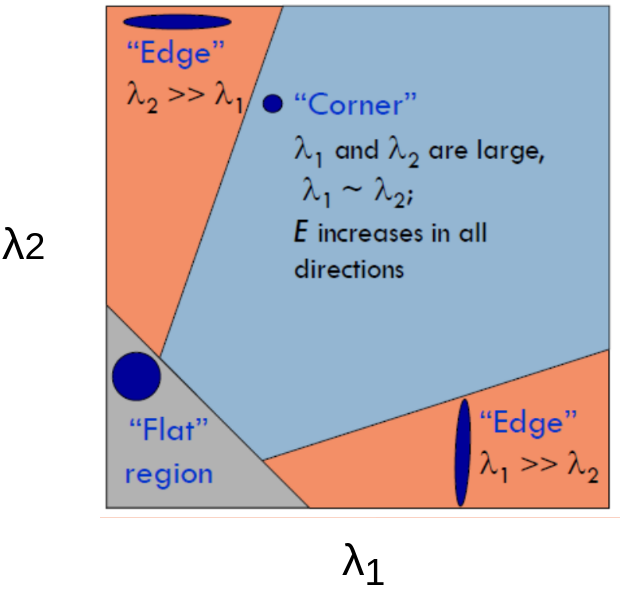
\includegraphics[scale=0.4]{img/eig2.png}
	\caption{Ilustración de cómo interpretar los valores de $\lambda_1$ y $\lambda_2$.}
	\label{fig:eig}
\end{figure}

Teniendo los valores anteriores para cada píxel, podemos calcular la media armónica
de un píxel, la cuál llamaremos $p$, de la siguiente forma:

\begin{equation}
	p	= \frac{\lambda_1 \lambda_2}{\lambda_1 + \lambda_2}
\end{equation}

Una vez dicho todo esto, vamos a ver cómo se podría implementar:

\begin{lstlisting}
def compute_points_of_interest(img, block_size, ksize):
    """
    Funcion que calucla los puntos de interes dada una imagen de entrada.
    Dichos puntos de interes son calculados mediante el operador de Harris.
    
    Args:
        img: Imagen de la que sacar los puntos de interes
        block_size: Tamaño del bloque que se va a tener en cuenta a la hora de
                    calcular los valores singulares.
        ksize: Tamaño del operador de Sobel
    Return:
        Devuelve una imagen del mismo tamaño que la entrada que contiene los
        puntos de interes calculados con el operador de Harris
    """
    # Obtener valores singulares y vectores asociados
    sv_vectors = cv2.cornerEigenValsAndVecs(img, block_size, ksize)

    # Quedarse solo con los valores singulares
    # Los valores singulares son los dos primeros valores de la matriz
    sv = sv_vectors[:, :, :2]

    # Calcular valor de cada pixel como \frac{lamb1 * lamb2}{lamb1 + lamb2}
    # Ahi donde el denominador sea 0, se pone un 0, para evitar que se calcule
    # un infinito
    prod_vals = np.prod(sv, axis=2)
    sum_vals = np.sum(sv, axis=2)
    points_interest = np.divide(prod_vals, 
        sum_vals,
        out=np.zeros_like(img),
        where=sum_vals!=0.0
    )

    return points_interest
\end{lstlisting}

Lo primero que hacemos es utilizar la función \texttt{cornerEigenValsAndVecs()} de
\texttt{OpenCV} para obtener los valores $\lambda_1$, $\lambda_2$ y los vectores
propios asociados a cada uno de los valores singulares de cada píxel de la imagen. Esto
nos dará de salida una matriz de las mismas dimensiones que la de entrada, pero
cada posición contendrá los 6 valores anteriormente dichos. Los parámetros que se
le pasan son \texttt{img}, que es la imagen de donde extraer la información,
\texttt{block\_size}, que indica cuál es el tamaño de la región alrededor del píxel
que se debe consultar para obtener los valores singulares, y \texttt{ksize}, que indica
el tamaño del \textit{kernel} de Sobel que va a utilizar la función.

A continuación nos quedamos solo con los valores singulares, los cuáles están situados en
las dos primeras posiciones. Calculamos la suma y el producto para cada par de $\lambda_1$
y $\lambda_2$, y después calculamos la media armónica. Para evitar problemas donde por
ejemplo el denominador es 0, la operación solo se realiza para aquellos valores en los que
el denominador sea distinto de 0. De esta forma, en las posiciones en las que no se dé,
se pondrá un 0, ya que se considerará que no ofrecen información relevante. Dicha operación
se puede ver en el código anterior en las líneas 27-31, donde en la línea 29 se declara que
la salida será una matriz inicialmente con ceros y en la 30 se especifica que la división solo se
haga en aquellas posiciones donde el denominador sea distinto de 0.

Una vez que hemos obtenido los puntos de Hrris, el siguiente paso es aplicar un umbral,
de forma que los píxels de la imagen resultante que están por debajo del valor umbral serán
eliminados, poniéndolos a 0. De esta forma, podemos eliminar aquellos puntos con valores
bajos, ya que la mayoría de ellos
estarán asociados a regiones planas, es decir, regiones donde la intensidad varíe muy poco,
y por tanto, donde los valores $\lambda_1$ y $\lambda_2$ sean bajos.
También es posible que en el proceso se elimine algún punto asociado a un borde que no sea muy importante,
aunque eso depende bastante del valor umbral que se utilice. En el \textit{paper} utilizaron un valor de
10, aunque nosotros probaremos luego con otros valores.

Para aplicar el umbral a la imagen, hemos hecho una función, la cuál se muestra a continuación:

\begin{lstlisting}
def threshold_points_of_interest(points, threshold):
    """
    Funcion que aplica un umbral sobre una imagen, poniendo los pixels por
    debajo del umbral a 0

    Args:
        points: Puntos/Imagen sobre la que aplicar la umbralizacion
        threshold: Valor umbral
    Return:
        Devuelve una imagen en la que los valores por debajo del umbral han
        sido puestos a 0
    """
    points[points < threshold] = 0.0
\end{lstlisting}

Lo único que se hace es encontrar las posiciones en las que el píxel tenga un valor inferior al umbral
y se pone dicho píxel a 0.

Posteriormente, tenemos que aplicar la supresión de no máximos, de forma que
eliminamos los valores que no sean máximos locales. De esta forma, eliminamos
valores que puedan estar asociados a ruido. El código es casi el mismo
que el utilizado en la práctica 1. La única diferencia es que ahora el tamaño de la
ventana está parametrizado, pero el funcionamiento sigue siendo el mismo que teníamos
anteriormente.

Una vez que hemos aplicado los pasos anteriores, los píxels que queden ``vivos'' en la
imagen son los que ofrecen información relevante sobre esta, ya que son aquellos que podríamos
decir que, en general, ofrecen información sobre las esquinas que se puedan encontrar en la imagen
a una escala determinada. Por tanto, podríamos tratar dichos puntos como descriptores
o \textit{keypoints}, aunque nos falta algo más de información. Tenemos que conocer,
aparte de la posición del punto, la escala en la que se ha detectado y su orientación.

Calcular la escala es algo trivial. Siguiendo las indicaciones proporcionadas, podemos calcular dicho
valor como $blockSize \times nivel\_piramide$, donde $blockSize$ es el tamaño del bloque que se
ha utilizado para calcular los valores de $\lambda_1$ y $\lambda_2$ para cada píxel, y
$nivel\_piramide$ es, como su propio nombre indica, el nivel actual de la pirámide.

No obstante, el cálculo de la orientación no es tan directo como en el caso anterior, ya que necesitamos
información sobre los gradientes de un punto determinado en una escala concreta. Afortunadamente, aquí es
donde entran en juego las pirámides Gaussianas que calculamos al principio para las derivadas
de la imagen, las cuales nos facilitan mucho la vida. Vamos a ver primero la implementación
y luego comentaremos lo que se hace:

\begin{lstlisting}
def compute_orientation(dx_grad, dy_grad):
    """
    Funcion que calcula la orientacion del gradiente de una serie de puntos

    Args:
        dx_grad: Derivadas en el eje X
        dy_grad: Derivadas en el eje Y
    Return:
        Devuelve un array en el que estan las orientaciones de todos los
        pares de gradientes de dx_grad y dy_grad. Las orientaciones estan
        en grados, y se encuentran en el rango [0, 360)
    """
    # Obtener vectores u y sus normas
    u = np.concatenate([dx_grad.reshape(-1,1), dy_grad.reshape(-1,1)], axis=1)
    u_norm = np.linalg.norm(u, axis=1)

    # Calcular vectores [cos \theta, sen \theta]
    vec_cos_sen = u / u_norm.reshape(-1, 1)
    cos_vals = vec_cos_sen[:, 0]
    sen_vals = vec_cos_sen[:, 1]

    # Calcular sen/cos arreglando posibles errores como 0/0 y x/0
    # Se arreglan los errores poniendolos a 0.0
    orientations = np.divide(sen_vals,
        cos_vals,
        out=np.zeros_like(sen_vals),
        where=cos_vals!=0.0
    )

    # Obtener \theta usando arcotangente (resultado en radianes
    # entre [-pi/2, pi/2])
    orientations_rad = np.arctan(orientations)

    # Obtener angulos y arreglarlos (sumar 180 grados en caso de que cos < 0
    # y pasarlos al rango [0, 360], eliminando negativos)
    orientations_degrees = np.degrees(orientations_rad)
    orientations_degrees[cos_vals < 0.0] += 180.0
    orientations_degrees[orientations_degrees < 0.0] += 360.0
    
    return orientations_degrees
\end{lstlisting}

La función recibe como parámetro las derivadas en el eje $X$ y en el eje $Y$ de los
puntos ``vivos'' de una escala determinada. Lo primero que hace es calcular el vector
de gradientes $\mathbf{u}$ asociado a cada par de de derivadas, el cuál viene dado
por $\mathbf{u} = [\frac{\partial I}{\partial x}, \frac{\partial I}{\partial y}]$. Se calcula
dicho vector para todas las parejas a la vez, ya que solo consiste en juntar las derivadas,
poniéndolas como vectores columna. También se calcula $\mathbf{|u|}$, que es la norma
euclídea de  $\mathbf{u}$.

Después, se divide cada vector  $\mathbf{u}_i$ entre su norma
$\mathbf{|u|}_i$, resultando en un vector donde tenemos que los valores son $[cos(\theta), sin(\theta)]$.
Estos valores son el coseno y el seno del ángulo $\theta$ que queremos calcular. De aquí
sacamos los valores de forma separada, para poder acceder a ellos de forma más
sencilla. Los cosenos están en la primera columna, y los senos en la segunda.

Ahora, para obtener la orientación, lo primero que tenemos que hacer es dividir
el seno entre el coseno para cada vector. De esta forma obtenemos $tan(\theta)$.
Esta operación puede verse en las líneas 24-28. De nuevo, tal y como pasaba en el
caso de los puntos de Harris, es posible que alguno de los senos sea 0. Para evitar
que el resultado no sea válido, se aplica la corrección vista anteriormente, donde
solo se realiza la operación allí donde el seno sea distinto a 0. En caso contrario,
la salida generada es 0.

A partir del resultado anterior ya podemos sacar el ángulo. Como el resultado
anterior es la tangente de $\theta$, podemos aplicar la función arco tangente, la
cuál es la inversa, para sacar el ángulo. El principal problema es que el valor
devuelto está en radianes, y está en el rango $[-\frac{\pi}{2}, \frac{\pi}{2}]$. Por tanto, tenemos
que pasar los ángulos de radianes a grados. Dicha transformación se realiza con una función de
\texttt{numpy}, la cuál es \texttt{degrees()}. Esta función pasará los valores a
grados, aunque estarán en el rango $[-90, 90]$. Por tanto, hay una serie
de operaciones extra que tenemos que hacer:

\begin{enumerate}
	\item Tenemos que identificar los puntos cuyo coseno sea negativo, ya que los valores
	obtenidos anteriormente se sitúan en el primer y en el cuarto cuadrante. Esto viene a raíz
	de que la tangente es positiva tanto en el primer como en el tercer cuadrante, y es negativa
	tanto en el segundo como en el cuarto cuadrante.  Por tanto, tenemos que ajustar los ángulos
	obtenidos. Para hacer esto, podemos guiarnos por el coseno, ya que este es positivo en el primer
	y cuarto cuadrante y negativo en los otros dos. Por tanto, simplemente tenemos que buscar los
	índices de los cosenos que sean negativos, y sumar a los ángulos en las mismas posiciones
	180, de forma que se ajusten al ángulo en el cuadrante que les corresponda.
	\item Puede que aun queden valores negativos porque están en el cuarto cuadrante. En un principio,
	esto no debería ser un problema, pero \texttt{OpenCV} exige que los grados estén en el rango
	$[0, 360)$. Por tanto, a todos los ángulos menores que 0, hay que sumarles 360.
\end{enumerate}

Después de todo este proceso, ya tenemos las orientaciones calculadas, y podríamos
proceder a la creación de \textit{keypoints} con la información que tenemos.

Para simplificar todo el proceso, hemos creado una única función que se encarga de
todo el proceso anterior. A continuación se puede ver el código de dicha función:

\begin{lstlisting}
def harris_corner_detection(img, block_size, window_size, ksize_der,
                            n_octaves, threshold=10.0):
    """
    Funcion que detecta los puntos de Harris de una imagen a distintas
    escaslas.

    Args:
        img: Imagen de la que se quieren extraer los puntos de Harris
        block_size: Tamaño del bloque que se va a tener en cuenta a la hora de
                    calcular los valores singulares.
        window_size: Tamaño de la ventana al realizar la supresion de no
                     maximos
        ksize_der: Tamaño del operador de Sobel (utilizado en el calculo
                   de los valores singulares)
        n_octaves: Numero de octavas/escalas de la imagen de la que sacar
                   puntos
        threshold: Umbral utilizado para eliminar todos los valores inferiores
                   a este.
    Return:
        Devuelve dos listas: una que contiene los keypoints extraidos y otra
        que contiene los keypoints corregidos
    """
    # Obtener piramide gaussiana de la imagen
    img_pyr = compute_gaussian_pyramid(img, n_octaves)

    # Obtener piramides de las derivadas
    dx_pyr, dy_pyr = compute_derivative_pyramids(img, ksize_der, n_octaves)

    # Lista de keypoints y keypoints corregidos
    keypoints = []
    corrected_keypoints = []

    for i in range(n_octaves):
        # Obtener puntos de interes de la escala
        points_interest = compute_points_of_interest(img_pyr[i],
            block_size,
            ksize_der
        )

        # Aplicar umbralizacion
        threshold_points_of_interest(points_interest, threshold)

        # Aplicar supresion de no maximos
        points_interest = non_max_supression(points_interest, window_size)

        # Obtener valores mayores que 0.0 (aquellos que no han sido eliminados)
        points_idx = np.where(points_interest > 0.0)

        # Calcular escala del KeyPoint
        # Hace falta incrementar el valor de i en 1 porque se empieza en 0
        scale = (i+1) * block_size

        # Obtener las derivadas correspondientes a los puntos no eliminados
        dx_grad = dx_pyr[i][points_idx]
        dy_grad = dy_pyr[i][points_idx]

        # Calcular orientaciones de los puntos no eliminados
        orientations = compute_orientation(dx_grad, dy_grad)

        # Lista que contiene los keypoints de la octava/escala
        # Se corrigen las coordenadas segun la escala
        keypoints_octave = [cv2.KeyPoint(x*2**i, y*2**i, scale, o)
                            for y, x, o in zip(*points_idx, orientations)]

        # Unir las coordenadas de forma que sean n vectores [x,y] formando una  
        # matriz
        points_x = points_idx[0].reshape(-1,1)
        points_y = points_idx[1].reshape(-1,1)
        points = np.concatenate([points_x, points_y], axis=1)

        # Establecer criterio de parada
        # Se parara o bien a las 15 iteraciones o cuando epsilon sea menor a 0.01
        criteria = (cv2.TERM_CRITERIA_EPS + cv2.TERM_CRITERIA_MAX_ITER, 15, 0.01)

        # Corregir keypoints
        points = cv2.cornerSubPix(img_pyr[i],
            points.astype(np.float32),
            (3,3),
            (-1,-1),
            criteria
        )

        # Redondear, cambiar x por y y viceversa (OpenCV carga las imagenes
        # invirtiendo los ejes) y transformar coordenada a la de la imagen original
        points = np.round(points)
        points = np.flip(points, axis=1)
        points *= 2**i

        # Guardar keypoints y keypoints corregidos
        keypoints.append(keypoints_octave)
        corrected_keypoints.append(points)

    return keypoints, corrected_keypoints
\end{lstlisting}

La función recibe como parámetros la imagen de la que sacar los puntos de Harris,
el tamaño de bloque utilizado en el cómputo de los valores singulares (tal y como
se ha explicado anteriormente), el tamaño de la ventana que se va a utilizar en la supresión
de no máximos el tamaño del \textit{kernel} de la derivada, el número de octavas o escalas
que se quieren sacar de la imagen (lo cuál determina el tamaño de las pirámides) y el
umbral que se tiene que aplicar para reducir el número de puntos. Por defecto, el
umbral está puesto a 10, que es el valor que se probó en el \textit{paper}.

Esta función, aparte de hacer todo lo especificado anteriormente, también se encarga
de corregir las posiciones de los \textit{keypoints} que se han obtenido, utilizando
para ello la función de \texttt{OpenCV} \texttt{cornerSubPix(...)}. De esta forma, realizamos
todos los cálculos a la vez, y no necesitamos repetir el proceso. Estos puntos serán utilizados
más adelante para comparar qué tal han salido los puntos estimados. De momento, vamos
a explicar lo que hace la función, y cuando aparezca la llamada a esta función nos
pararemos a explicarla más detenidamente.

Lo primero que hace la función es obtener las pirámides de la imagen y de las derivadas,
además de crear las listas que contendrán la información de salida.

Una vez hecho esto, repite todos los pasos descritos anteriormente tantas veces como
octavas/escalas se le hayan especificado. Primero extrae los puntos de Harris, después
elimina los que están por debajo del umbral y realiza la supresión de no máximos. Una vez
hecho esto, determina las posiciones en las que los puntos tienen un valor superior a 0 y
las guardan. Después, se encarga de calcular la escala y las orientaciones de la forma
descrita anteriormente. Con la información que ha extraído, crea los \textit{keypoints} de la escala,
lo cuál se puede ver en las líneas 62-63. Es importante destacar que, a la hora
de crear los \textit{keypoints}, se cambian las $x$ por las $y$ y viceversa. Esto se
hace así porque si no, a la hora de pintar los \textit{keypoints} posteriormente, estos
saldrán girados, ya que \texttt{OpenCV} carga las imágenes invirtiendo los ejes. Por tanto,
necesitamos invertir las posiciones manualmente para que posteriormente se puedan ver
bien. También es importante destacar que las coordenadas se multiplican por $2^i$, donde
$i$ es la octava/escala actual. Esto se debe a que, por ejemplo, al pasar de la base de la pirámide
al siguiente nivel,
lo que originalmente estaba en la posición $(x, y)$ ahora estará en la $(\frac{x}{2}, \frac{y}{2})$.
En el siguiente nivel estará en la posición $(\frac{x}{4}, \frac{y}{4})$, y así sucesivamente.
Esto se debe a que la imagen se va reduciendo la mitad en cada eje a medida que se
va subiendo de nivel en la pirámide Gaussiana. Por tanto, como las coordenadas obtenidas
son relativas a las de la imagen de una escala determinada, tenemos que adaptarlas a
las de la imagen original multiplicando por este factor.

Una vez que se han extraído los \textit{keypoints}, comienza el proceso en el que se
refinan. Para ello, lo primero que se hace es juntar las coordenadas obtenidas en una única
matriz, la cuál va a tener dos columnas: una para el eje $X$ y una para el $Y$. Después
de eso, establecemos el criterio de parada del método de refinamiento, el cuál es una tupla
que contiene los \textit{flags} y los valores. Con los \textit{flags} se indica que se parará o
bien cuando se pase un número de épocas o cuando el movimiento a la hora de refinar
en alguna época sea menor a un $\varepsilon$ dado. En este caso, se especifica que como máximo se hagan 15
iteraciones o el refinamiento se mueva menos de $\varepsilon = 0.01$. De esta forma,
no hacemos muchas iteraciones, y el valor de $\varepsilon$ se ha considerado como
el adecuado, ya que si se mueve menos que eso, significa que hemos encontrado
una posición muy próxima al mejor lugar, y se ha considerado suficiente el poco
margen de error que deja. Además, al tener tan pocas iteraciones límite, es difícil
ajustar mejor.

Con el criterio ya definido llamamos a la función \texttt{cornerSubPix},
la cuál recibe la imagen, las posiciones iniciales de los puntos que tiene que
refinar(los cuáles hemos obtenido antes), el tamaño de la ventana (el
valor que recibe es la \textbf{mitad} del tamaño total de la ventana), la región
alrededor del píxel en la que no buscar (la mitad de esta, igual que en el caso
anterior) y el criterio de parada. En este caso, para el tamaño de la ventana hemos
especificado que se use $(3,3)$, de forma que se busque en una región $7 \times 7$
alrededor del centro, ya que se ha estimado suficiente teniendo en cuenta los tamaños
de bloque que se usarán más adelante, los cuáles en ningún caso serán mayores que 5
debido a que el tamaño de la imagen se reduce demasiado rápido a medida que vamos
subiendo niveles en la pirámide Gaussiana. En cuanto a la región alrededor de píxel
en la que no buscar, he especificado $(-1,-1)$, de forma que se busque en toda la región,
ya que se ha considerado que no es buena idea limitar el poco espacio de búsqueda que
tenemos, ya que de por sí es pequeño.

Una vez que se obtienen los puntos refinados, se redondean los valores al entero más
próximo, se cambian las $x$ por las $y$ y viceversa (línea 86) y se escalan los valores
de las coordenadas a los de la imagen original.

Finalmente, se guardan tanto los \textit{keypoints} obtenidos como las posiciones
refinadas en las listas correspondientes, y se repite todo el proceso para el número
de octavas/escalas que se haya especificado.

\subsection{Experimentación con los parámetros}

Una vez que hemos descrito cómo se ha llevado a cabo todo el proceso, vamos
a experimentar un poco con los parámetros para ver qué \textit{keypoints} se
obtienen.

Para hacer las pruebas, vamos a utilizar la imagen \textit{Yosemite1.jpg}. Vamos
a extraer los \textit{keypoints} en la imagen en blanco y negro y los pintaremos
sobre la imagen en color. Vamos a probar a variar el tamaño del bloque, el tamaño
del \textit{kernel} de las derivadas, el el tamaño de la ventana y el umbral. En todos
los casos utilizaremos 5 escalas, ya que se ha considerado un número adecuado. En
caso de haber escogido más, la imagen se hubiese quedado muy pequeña en los últimos
niveles, y con menos, a lo mejor se perdía detalle. Con la mejor combinación de parámetros
se mostrará un desglose de los \textit{keypoints} por escalas.

El caso base será uno en el que se use un tamaño de bloque de 5, un tamaño de ventana
y de \textit{kernel} de derivada 3, 5 escalas y un umbral de 10. El tamaño del bloque se ha escogido
de 5 ya que la imagen decrece muy rápido de tamaño, con lo cuál coger uno más grande no tiene mucho
sentido. El tamaño de la ventana se ha cogido de 3 porque se cree que es suficiente, ya que busca
en una región más o menos pequeña cuál, de forma que no es influido por píxels que están
más lejos del actual. Se ha estimado que un tamaño de \textit{kernel} para las derivadas
de 3 es suficiente, ya que suele ofrecer buenos resultados. En cuanto al umbral, se ha dejado
el umbral por defecto, ya que es el que venía en el \textit{paper}. 

En cada caso, se indicará cuáles son los parámetros modificados y cuántos puntos se
han detectado a lo largo de todas las escalas. A continuación se pueden ver los resultados:

\begin{figure}[H]
	\centering
	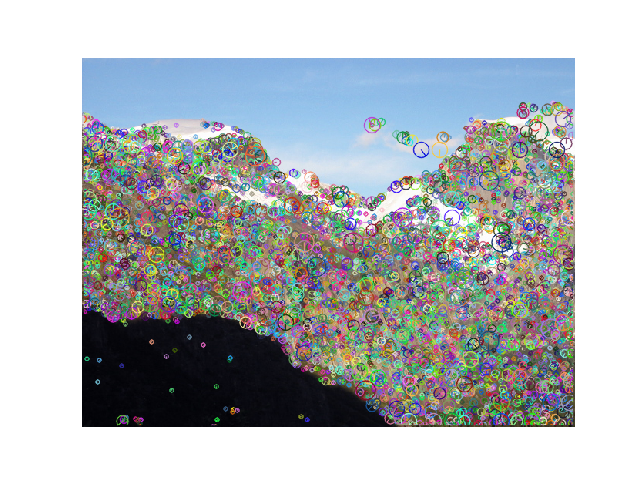
\includegraphics[scale=0.6]{img/kp-base}
	\caption{\textit{Keypoints} obtenidos para el caso base. 6731 puntos detectados.}
	\label{fig:kp-base}
\end{figure}

\begin{figure}[H]
	\centering
	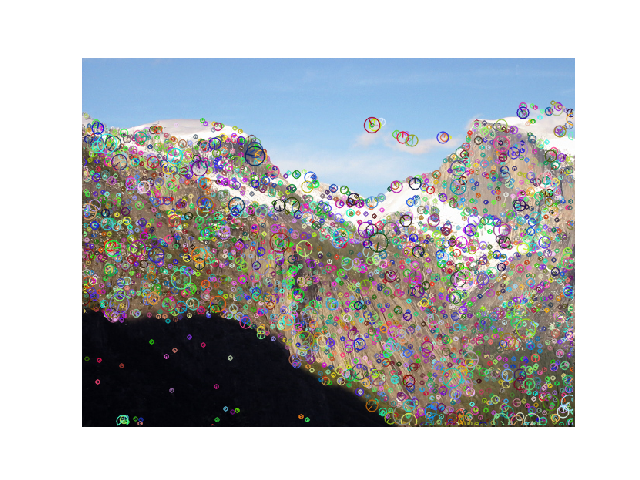
\includegraphics[scale=0.6]{img/kp-window}
	\caption{\textit{Keypoints} obtenidos con tamaño de ventana de 5. 2982 puntos detectados.}
	\label{fig:kp-window}
\end{figure}

\begin{figure}[H]
	\centering
	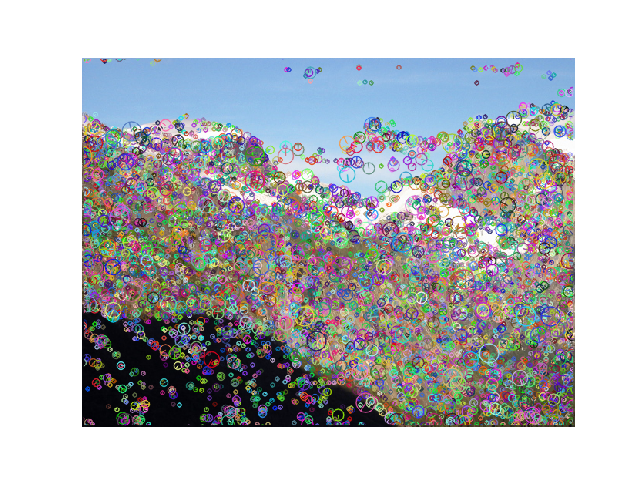
\includegraphics[scale=0.6]{img/kp-der}
	\caption{\textit{Keypoints} obtenidos con tamaño del \textit{kernel} de derivadas de 5. 6911 punto detectados.}
	\label{fig:kp-der}
\end{figure}

\begin{figure}[H]
	\centering
	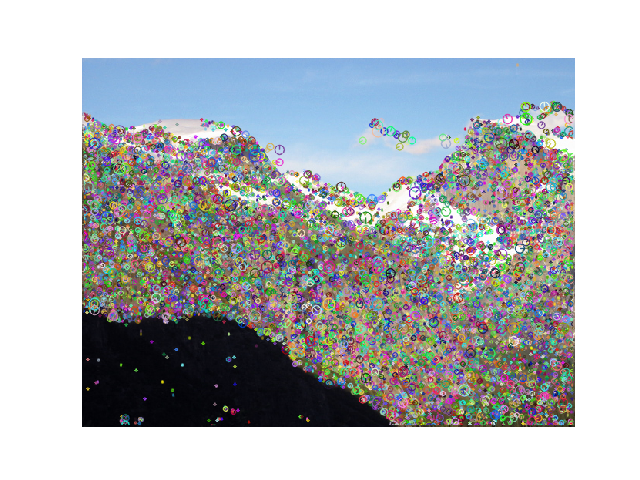
\includegraphics[scale=0.6]{img/kp-block}
	\caption{\textit{Keypoints} obtenidos con tamaño de bloque de 3. 11013 puntos detectados.}
	\label{fig:kp-block}
\end{figure}

\begin{figure}[H]
	\centering
	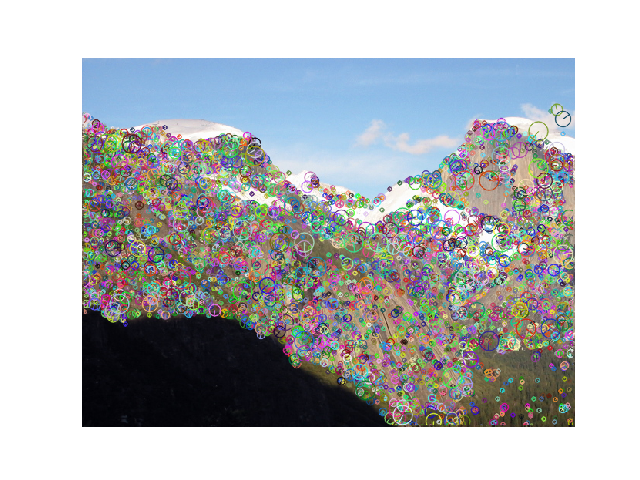
\includegraphics[scale=0.6]{img/kp-thresh60}
	\caption{\textit{Keypoints} obtenidos con umbral de 60. 5610 puntos detectados.}
	\label{fig:kp-thresh60}
\end{figure}

\begin{figure}[H]
	\centering
	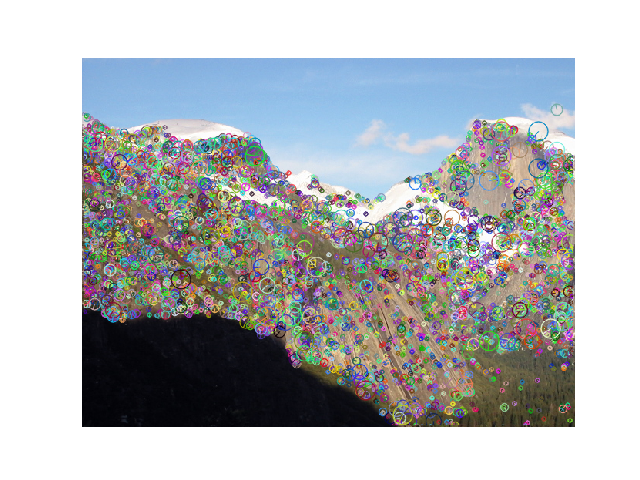
\includegraphics[scale=0.6]{img/kp-thresh90}
	\caption{\textit{Keypoints} obtenidos con  umbral de 90. 5113 puntos detectados.}
	\label{fig:kp-thresh90}
\end{figure}

\begin{figure}[H]
	\centering
	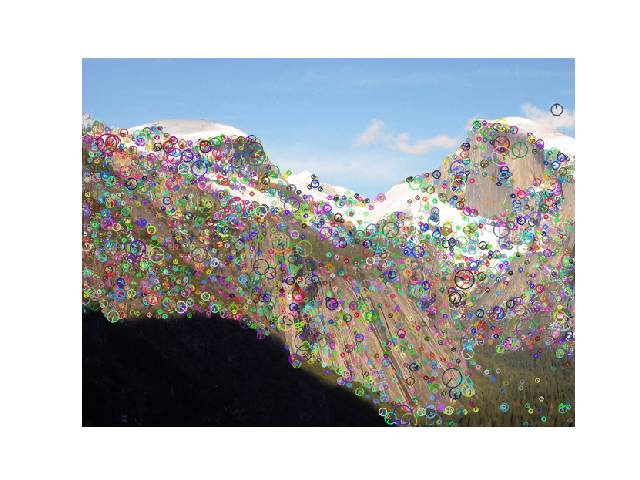
\includegraphics[scale=0.6]{img/kp-wind-thresh}
	\caption{\textit{Keypoints} obtenidos con ventana de tamaño 5 y umbral de 90. 2460 puntos detectados.}
	\label{fig:kp-wind-thresh}
\end{figure}

Observando los resultados de forma general, podemos ver que en todos los casos se
obtienen más de 2000 \textit{keypoints}. Parece que, en general, disminuir el tamaño
del bloque y aumentar el tamaño del \textit{kernel} de la derivada hacen que se detecten
más puntos que en el caso base. En el primer caso, esto parece lógico, ya que se tienen en
cuenta menos píxels para determinar la variación de la intensidad, y por tanto, las estimaciones
se quedan bastante más cortas, ya que posiblemente si se utilizase un entorno mayor, los valores
singulares hubiesen sido más pequeños. En el segundo caso, puede deberse a que el operador
haga que las variaciones de intensidad sean más notables, ya que ponderaría más a los píxels
cercanos al centro. Por tanto, estaría de alguna forma sobreestimando de alguna forma las variaciones,
aunque tampoco estamos muy seguros de que sea esto lo que suceda.

Si en cambio aumentamos el tamaño de la ventana o el del umbral, como es lógico, el número
de \textit{keypoints} se ve disminuido. Este descenso es mucho más drástico cuando se aumenta
el tamaño de la ventana, ya que se eliminan más puntos debido a que se considera
un entorno mucho mayor a la hora de buscar el máximo de la región. Por tanto, encontraremos
valores que antes no habíamos considerado dentro de la región, y que por tanto, harán que lo
que antes era un máximo local deje de serlo. Esto sin embargo presenta un pequeño problema, y es
que no debemos abusar del tamaño de la ventana: un tamaño demasiado grande nos puede hacer
perder demasiados puntos. Por tanto, lo suyo sería intentar coger, como mucho, una ventana con las
mismas dimensiones que el tamaño del bloque utilizado, de forma que se busque el máximo en el entorno
de donde se han extraído los valores singulares.  Si en vez de aumentar el tamaño de la ventana
aumentamos el umbral, tal y como dijimos antes, también se reducen el número de puntos encontrados.
Esto se debe a que se exige que los valores singulares sean más grandes, y que por tanto,
que las variaciones en intensidad sean más pronunciadas. Por tanto, estamos haciendo que
la detección sea algo más robusta, ya que buscamos las esquinas más destacables. Aunque,
igual que en el caso anterior, no debemos abusar del umbral, ya que uno muy grande nos puede hacer
empezar a perder puntos que pudiesen ser clave.

Vemos que si combinamos tanto el incremento del umbral como el aumento del tamaño de la
ventana, como se ha hecho en la figura \ref{fig:kp-wind-thresh},  obtenemos un conjunto de
\textit{keypoints} que parece ser razonable, ya que son más de 2000, pero no es un número
excesivamente grande. Además de eso, parece que se dejan de detectar algunos puntos que
no tenían mucho sentido. Por ejemplo, no se detectan los puntos de la zona oscura, los cuáles
sí que se detectaban cuando solo se aumentaba el tamaño de la ventana, y no se detectaban
al aumentar umbral. Estos puntos no tenían mucho sentido, ya que realmente no hay ninguna
esquina ahí y no parece que pueda ofrecer mucha información. Además, a simple vista,
aunque haya cierta variación de la intensidad, esta no es muy significativa.

Para dibujar los \textit{keypoints} anteriores se ha utilizado la siguiente función:

\begin{lstlisting}
def draw_all_keypoints(img, keypoint_list):
    """
    Funcion que dibuja todos los keypoints detectados

    Args:
        img: Imagen sobre la que pintar los keypoints
        keypoint_list: Lista con los keypoints
    """
    # Juntar los keypoints de todas las escalas
    keypoints= [k for keypoints_octave in keypoint_list for k in keypoints_octave]

    # Transformar imagen a uint8 y RGB
    vis = transform_img_uint8_RGB(img)

    # Crear imagen de salida vacia del mismo tamaño que la original
    out = np.empty_like(vis)

    # Dibujar keypoints
    out = cv2.drawKeypoints(vis,
        keypoints,
        out,
        flags=cv2.DRAW_MATCHES_FLAGS_DRAW_RICH_KEYPOINTS
    )

    # Visualizar la imagen
    visualize_image(out)
\end{lstlisting}

Esta función recibe la imagen sobre la que se quieren pintar los \textit{keypoints} y
una lista con todos los puntos extraídos. Lo primero que hace es juntar todos los
\textit{keypoints} extraídos a distintas escalas en una única lista. Después 
transforma la imagen a entero sin signo y al formato RGB, ya que se usa \texttt{matplotlib}. Es necesario que la
imagen esté en entero sin signo, ya que la función \texttt{drawKeypoints} obliga
a que sea de este tipo para poder pintar los \textit{keypoints}. Después
de esto, se crea una imagen de salida, la cuál inicialmente está vacía, y que es
donde escribirá el resultado. Finalmente, se pinta cada \textit{keypoint} sobre
la imagen se salida utilizando la función  \texttt{drawKeypoints}, a la cuál
se le pasa la imagen de entrada, los puntos, la imagen de salida, y un \textit{flag},
que en este caso indica que se pinten los \textit{keypoints} utilizando un formato
rico en el que se muestran círculos de distintos colores, escalas y orientaciones.

Una vez que hemos comentado esto, vamos a mostrar ahora los \textit{keypoints} que
se han detectado en cada escala para alguno de los casos anteriores. En este caso,
vamos a utilizar los puntos que se pueden ver en la figura \ref{fig:kp-wind-thresh}, ya
que se considera que es el mejor conjunto de \textit{keypoints} que se han extraído,
tanto porque no son demasiados como porque parecen ser relevantes, sin incluir
puntos que puedan aportar poca o nula información.

Para dibujar dichos puntos nos hemos ayudado de la siguiente función:

\begin{lstlisting}
def draw_keypoints_octave(img, keypoint_list):
    """
    Funcion que dibuja los keypoints por cada escala

    Args:
        img: Imagen sobre la que pintar los keypoints
        keypoint_list: Lista con los keypoints
    """
    # Transformar imagen a uint8 y RGB
    vis = transform_img_uint8_RGB(img)

    for keypoints in keypoint_list:
        # Crear imagen de salida vacia del mismo tamaño que la original
        out = np.empty_like(vis)

        # Dibujar keypoints de la octava
        out = cv2.drawKeypoints(vis,
            keypoints,
            out,
            flags=cv2.DRAW_MATCHES_FLAGS_DRAW_RICH_KEYPOINTS
        )

        # Visualizar la imagen
        visualize_image(out)
\end{lstlisting}

La función es muy parecida a la que teníamos antes. Lo único que cambia es que no juntamos
\textit{keypoints} en una única lista y que pintamos de forma individual los \textit{keypoints}
de cada escala.

Una vez dicho esto, vamos a ver qué puntos hemos detectado en cada escala:

\begin{figure}[H]
	\centering
	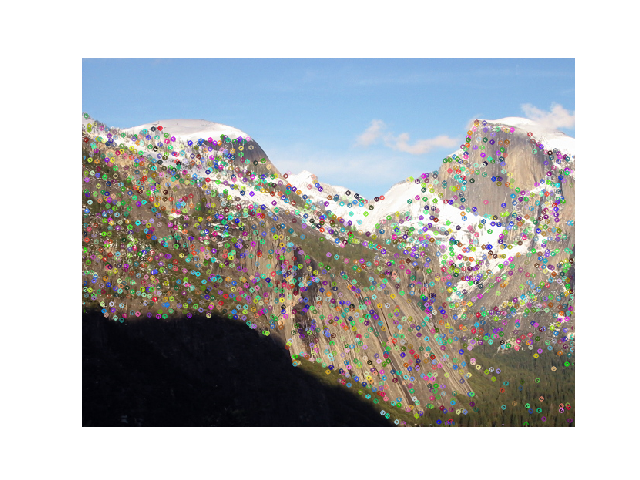
\includegraphics[scale=0.6]{img/scale0}
	\caption{\textit{Keypoints} detectados en el primer nivel.}
	\label{fig:scale0}
\end{figure}

\begin{figure}[H]
	\centering
	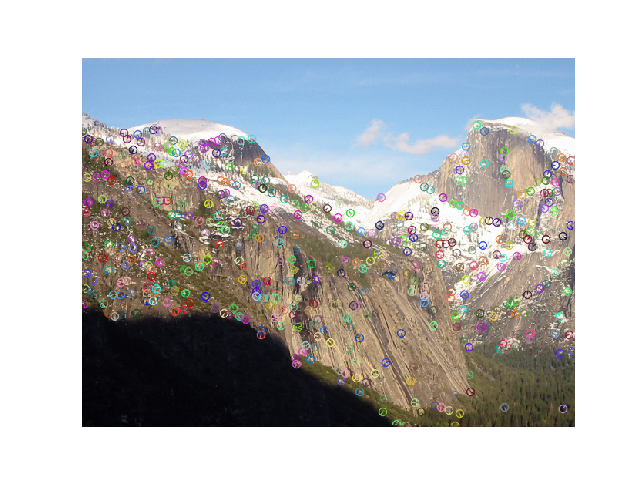
\includegraphics[scale=0.6]{img/scale1}
	\caption{\textit{Keypoints} detectados en el segundo nivel.}
	\label{fig:scale1}
\end{figure}

\begin{figure}[H]
	\centering
	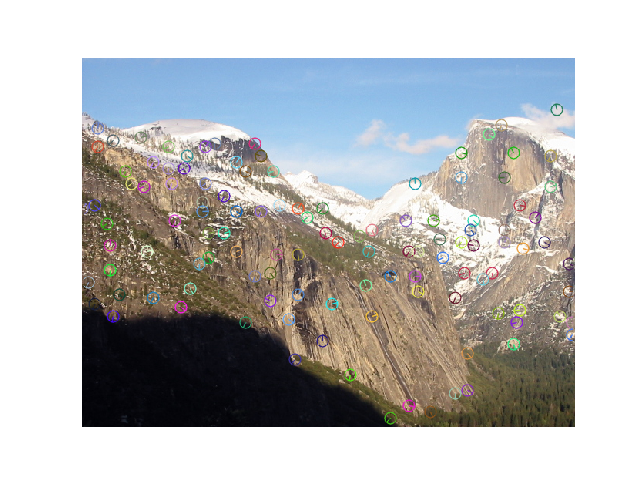
\includegraphics[scale=0.6]{img/scale2}
	\caption{\textit{Keypoints} detectados en el tercer nivel.}
	\label{fig:scale2}
\end{figure}

\begin{figure}[H]
	\centering
	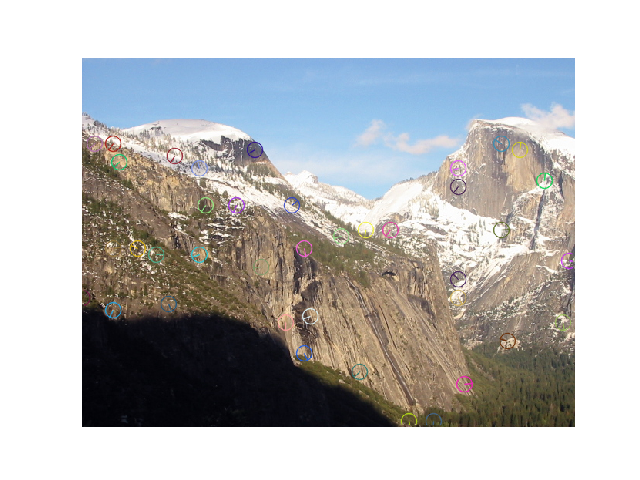
\includegraphics[scale=0.6]{img/scale3}
	\caption{\textit{Keypoints} detectados en el cuarto nivel.}
	\label{fig:scale3}
\end{figure}

\begin{figure}[H]
	\centering
	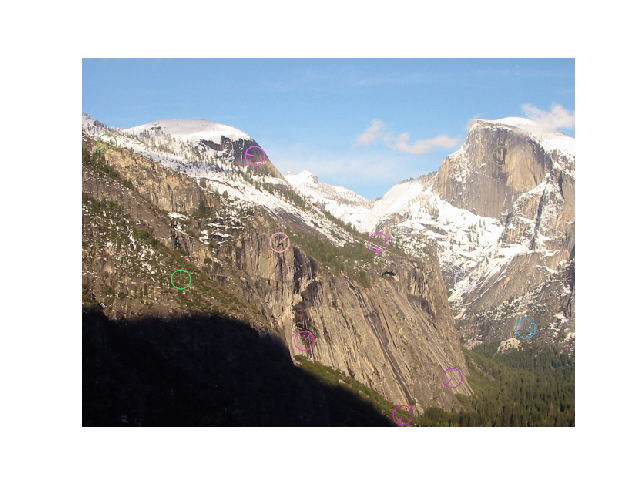
\includegraphics[scale=0.6]{img/scale4}
	\caption{\textit{Keypoints} detectados en el quinto nivel.}
	\label{fig:scale4}
\end{figure}

Vemos que, a medida que extraemos \textit{keypoints} de niveles más elevados
de la pirámide, el número que extraemos es cada vez menor, ya que al hacerse la
imagen cada vez más pequeña, el número píxels que pueden ser un \textit{keypoint}
son cada vez menos. En general, la evolución es pasar de tener muchos \textit{keypoints}
bastante juntos dentro de una zona determinada de la imagen a tener pocos puntos bastante separados unos de otros.
Esto es un efecto directo de la escala, ya que en los niveles más bajos nos permite fijarnos
en los detalles generales y, a medida que vamos aumentando la escala, nos permite fijarnos
en detalles más específicos y/u ocultos. Ya que los detalles generales son más abundantes,
vamos a encontrar más de estos que de los que son más específicos, lo cuál también explica por
qué vamos encontrando cada vez menos y menos (además de lo que hemos mencionado previamente
del tamaño de las imágenes).

Por tanto, es importante que al realizar
la extracción de descriptores, este proceso se haga en múltiples escalas, ya que
permite extraer información de distintas partes de la imagen de forma efectiva.
Hacerlo con una única escala no nos permitiría obtener toda la información a la primera,
ya que es muy difícil sacarla toda con una sola pasada en  una única escala.

\subsection{Comparación de la estimación con los puntos refinados}

Por último, para concluir este ejercicio, vamos a estudiar

\section{\textsc{Extracción de descriptores AKAZE}}

\section{\textsc{Mosaico de dos imágenes}}

\section{\textsc{Mosaico de \textit{N} imágenes}}

\newpage

\bibliographystyle{plain}
\bibliography{mybib}

\end{document}

